\chapter{Mass fit to \decay{\Bp}{\Dsp\Kp\Km} candidates} 
\label{ch:B2DsKK}

\minitoc

In this chapter the methodology used to search for \decay{\Bp}{\Dsp\Kp\Km} decays is described.
The branching fraction $\BF(\decay{\Bp}{\Dsp\Kp\Km})$ is determined by measuring the ratio of \decay{\Bp}{\Dsp\Kp\Km} and \decay{\Bp}{\Dsp\Dzb} yields. 
This is corrected by the ratio of efficiencies for the two modes and multiplied by the externally measured branching fractions for \decay{\Bp}{\Dsp\Dzb} and \decay{\Dzb}{\Kp\Km} decays.

\begin{multline}
\BF(\decay{\Bp}{\Dsp\Kp\Km}) = \frac{N(\decay{\Bp}{\Dsp\Kp\Km})}{N(\decay{\Bp}{\Dsp\Dzb})} \times  \frac{\epsilon(\decay{\Bp}{\Dsp\Dzb})}{\epsilon(\decay{\Bp}{\Dsp\Kp\Km})}\\ 
\times \BF(\decay{\Bp}{\Dsp\Dzb}) \times \BF(\decay{\Dzb}{\Kp\Km}) 
\end{multline}

The fit models used to extract the yields $N(\decay{\Bp}{\Dsp\Kp\Km})$ and $N(\decay{\Bp}{\Dsp\Dzb})$ are described in Section~\ref{sec:B2DsKK_fitcomps}, the efficiency corrections are described in Section~\ref{sec:B2DsKK_effcorrection} and the resulting calculation of the branching fraction is in Section~\ref{sec:B2DsKK_results}.


\section{Fit components}
\label{sec:B2DsKK_fitcomps}

In order to extract the yields of \decay{\Bp}{\Dsp\Dzb} and \decay{\Bp}{\Dsp\Kp\Km} decays the invariant mass distributions for the processes contributing within the invariant mass range are parametrised with probability density functions (PDFs).

{\color{Red}
\begin{itemize}
\item mention fit range
\item any other quantities that might be needed
\end{itemize}
}


\subsection{Signal and normalisation decays}
\label{sec:B2DsKK_sigcomps}

The invariant mass distribution of \decay{\Bp}{\Dsp\Dzb} and \decay{\Bp}{\Dsp\Kp\Km} decays are parametrised as the sum of two Crystal Ball (CB) functions.
The CB function consists of a Gaussian function with a power-law tail and is typically used to parametrise losses due to radiative processes.
This is defined as
\begin{equation}
\text{CB}(m,\mu,\sigma,n,\alpha) = \left \{
  \begin{aligned}
    &e^{-\frac{1}{2} \left(\frac{m-\mu}{\sigma}\right)^2}, && \text{if}\ \left(\frac{m-\mu}{\sigma}\right) < -|\alpha|\\
    &\frac{\left(\frac{n}{|\alpha|}\right)^n\times e ^{-\frac{1}{2}|\alpha|^2} }{\left(\frac{n}{|\alpha|}-|\alpha| - \frac{m-\mu}{\sigma}\right)^n}, && \text{otherwise}
  \end{aligned} \right.
\end{equation} 

where $\mu$, $\sigma$, $n$ and $\alpha$ are adjustable parameters and $m$ is the \B meson invariant mass observable.

The sum of two CB functions is constructed with a variable fraction $f_\sigma$ assigned to the CB function with the narrower width,
\begin{equation}
\text{DCB}(m,\mu,\sigma_1,\sigma_2,n,\alpha) = f_\sigma \times \text{CB}(m,\mu,\sigma_1,n,\alpha) + (1-f_\sigma) \times \text{CB}(m,\mu,\sigma_2,n,\alpha),
\label{eq:DoubleBD}
\end{equation}
where the same tail parameters, $n$ and $\alpha$ are used for both functions, but the widths, $\sigma_1$ and $\sigma_2$, are allowed to be different (with $\sigma_1 < \sigma_2$).
As both CB shapes have the same parameter $\alpha$, the tails are constrained to be on the same side.
Values for the adjustable parameters are determined from fits to simulated decays passing the selection requirements applied to the data. These are determined separately for the different \Dsp decay modes. However, a number of parameters are not completely constrained from the simulations. The mean position $\mu$ is allowed vary freely in the fit to data, as is the narrowest CB width of the normalisation decay. The ratios $\sigma_1/\sigma_2$ and $\sigma_{1}(\Dsp\phi) / \sigma_{1}(\Dsp\Dzb)$ are fixed from simulations.
The tail parameters $n$ and $\alpha$ are highly correlated, therefore the value of $n$ is fixed to unity in both the fits to simulations and data. 



%%%%%%%%%%%%%%%%%%%%%%%%%%%%%%%%%%%%%%%%%%%%%%%%%%%%%%%%%% 
\begin{table}[h]
\centering
\begin{tabular}{ c c c c }
\hline
\multirow{2}{*}{Parameter}                   & \multicolumn{3}{c} {Value} \\
\cline{2-4}
                            & $\Dsp \to KK\pi$   & $\Dsp \to K\pi\pi$ & $\Dsp \to \pi\pi\pi$   \\
\hline
%\textbf{$\B \to \Ds \phi$}  &                    &                    &                        \\
\multicolumn{4}{l} {\decay{\Bp}{\Ds \phiz}}\\

\hline
$\sigma_1/\sigma_2$         & 0.49 $\pm$ 0.01    & 0.47 $\pm$ 0.01    & 0.46 $\pm$ 0.01        \\
$f_\sigma$                  & 0.80 $\pm$ 0.01    & 0.84 $\pm$ 0.01    & 0.81 $\pm$ 0.01        \\
$\alpha$                    & 2.76 $\pm$ 0.07    & 3.06 $\pm$ 0.16    & 3.71 $\pm$ 0.23        \\
$n$                         & 1 $\pm$ 0          & 1  $\pm$ 0         & 1  $\pm$ 0             \\
\hline
%\textbf{ }  &                    &                    &                        \\
\multicolumn{4}{l} {\decay{\Bp}{\Dsp\Dzb}}\\
\hline
$\sigma_1/\sigma_2$         & 0.43 $\pm$ 0.01    & 0.42 $\pm$ 0.01    & 0.40 $\pm$ 0.01        \\
$f_\sigma$                  & 0.88 $\pm$ 0.01    & 0.88 $\pm$ 0.01    & 0.88 $\pm$ 0.01        \\
$\alpha$                    & 2.91 $\pm$ 0.06    & 3.36 $\pm$ 0.26    & 3.53 $\pm$ 0.25        \\
$n$                         & 1 $\pm$ 0          & 1 $\pm$ 0          & 1 $\pm$ 0              \\
\hline 
$\sigma_{1}(\Dsp\phi) / \sigma_{1}(\Dsp\Dzb)$ & 1.27 $\pm$ 0.02 & 1.31 $\pm$ 0.02 & 1.26 $\pm$ 0.02 \\
\hline

\end{tabular}
\caption{Fixed values obtained in fits to MC used in the model for the signal pdf.} 
\label{tab:mc_fits}  
\end{table}
%%%%%%%%%%%%%%%%%%%%%%%%%%%%%%%%%%%%%%%%%%%%%%%%%%%%%%%%%% 

{\color{Red}
\begin{itemize}
\item plots of signal and normalisation fits
\end{itemize}
}

\subsection{Partially reconstructed backgrounds}
\label{sec:B2DsKK_partrecocomps}

Partially reconstructed decays are those in which the five final state particles combined in the signal mode are only a subset of a background mode's final state.
Decays of \B mesons can contribute at lower invariant masses below the signal peak when one or more the decay products have not been reconstructed. 
For decays to contribute within the fitted \Bp invariant mass window, the particle or particles that have not been reconstructed must be fairly low-momentum (soft) such that the invariant mass of the remaining particles is large.

\subsubsection{Backgrounds to the normalisation channel}

The low invariant mass region of the \Dsp\Dzb spectrum is populated by decays of \Bp mesons to combinations of \D and excited \D mesons. These \Dstarzb and \Dss mesons decay strongly to a ground state \Dzb or \Dsp meson and a soft pion or photon. The branching fractions for these decays are listed in Table~\ref{tab:dstar_BFs}.


%%%%%%%%%%%%%%%%%%%%%%%%%%%%%%%%%%%%%%%%%%%%%%%%%%%%%%%%%% 
\begin{table}[h]
\centering
\begin{tabular}{ l c }

\hline
Decay                           & Branching fraction \\ 
\hline
\decay{\Dstarzb}{\Dzb\Pgamma}   &   $(64.7\pm0.9)\%$ \\
\decay{\Dstarzb}{\Dzb\piz}      &   $(35.3\pm0.9)\%$ \\
\decay{\Dssp}{\Dsp\Pgamma}        &   $(93.5\pm0.7)\%$ \\
\decay{\Dssp}{\Dsp\piz}           &   $(5.8\pm0.7)\%$ \\
\hline

\end{tabular}
\caption{Branching fractions for excited charm mesons \cite{PDG2016}. } 
\label{tab:dstar_BFs}  
\end{table}
%%%%%%%%%%%%%%%%%%%%%%%%%%%%%%%%%%%%%%%%%%%%%%%%%%%%%%%%%% 

The excited charm mesons \Dstarzb and \Dss (be more specific) are vector ($J^{P} = 1^{-}$) mesons. The partially reconstructed invariant mass of the \Dsp and \Dzb mesons can vary depending on the spin of the missed particle.
analytical PDFs are used to account for the spin of the missed particle. These were developed by considering the 

{\color{Red}
\begin{itemize}
\item add formulas for hills and horns
\end{itemize}
}



\subsubsection{Backgrounds to the signal channel}

{\color{Red}
\begin{itemize}
\item plots of part reco shapes
\end{itemize}
}

\subsection{Combinatorial  background}
\label{sec:B2DsKK_combcomps}

The dominant source of background under the signal peak is due to combinations of unrelated tracks. This combinatorial background is modelled using an exponential function with a single degree of freedom controlling the effective slope of the shape. 

{\color{Red}
\begin{itemize}
\item check what happens to the slopes
\end{itemize}
}
This slope is shared between the normalisation and signal channels, and between different \Dsp decay modes. This adds stability to the fit.


\section{Fit strategy}
\label{sec:B2DsKK_fitstrategy}

{\color{Red}
\begin{itemize}
\item Single fit to signal and normalisation
\item $m(\Kp\Km)$ range that goes into fit
\item 
\end{itemize}
}



\section{Fit validation}
\label{sec:B2DsKK_fitvalidation}

{\color{Red}
\begin{itemize}
\item Toys for signal and normalisation
\item why it doesnt matter that norm yield have wrong pulls
\item 
\end{itemize}
}

\section{Normalisation and signal fits}


%%%%%%%%%%%%%%%%%%%%%%%%%%%%%%%%%%%%%%%%%%%%%%%%%%%%%%%%%%
\begin{figure}[!h]
    \centering
    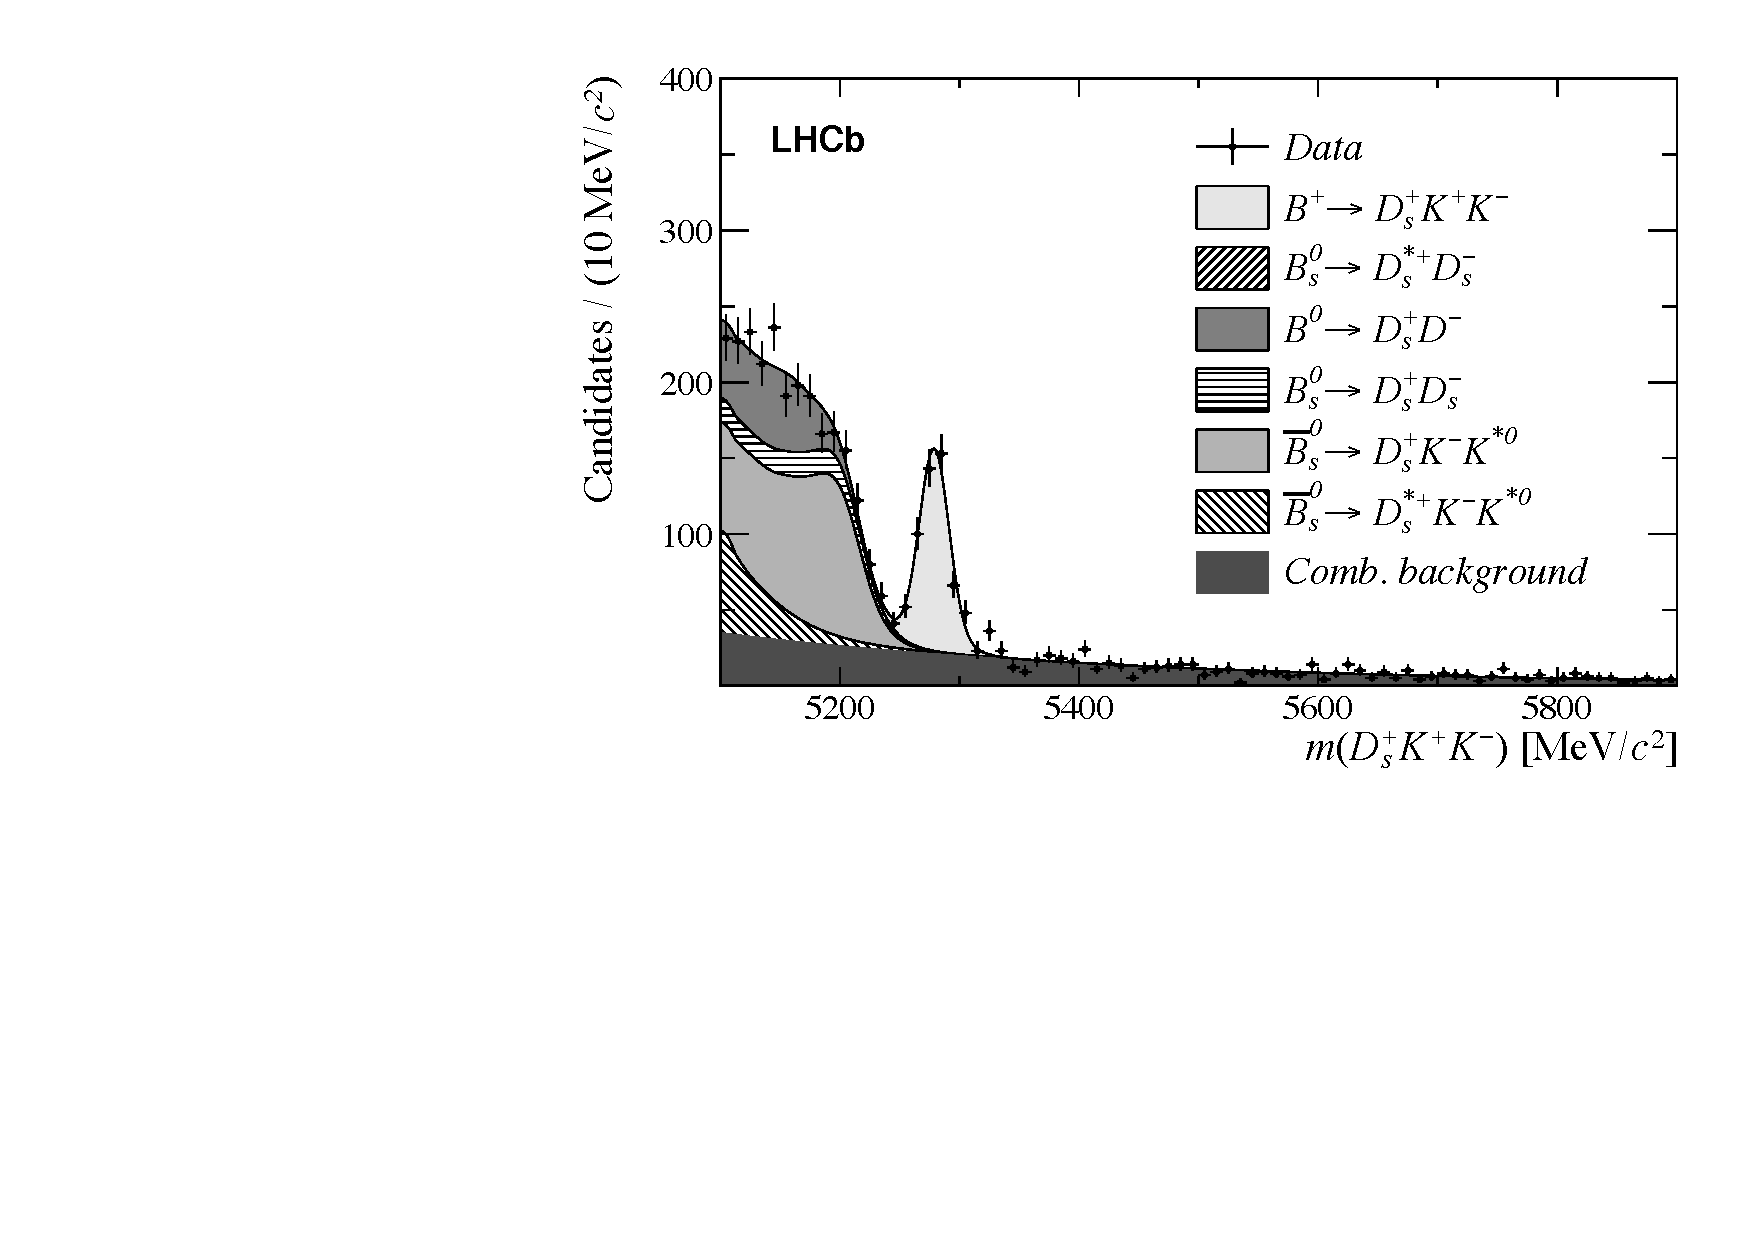
\includegraphics[width=0.8\textwidth]{figs/B2DsKK/Fit_DsKK_BandW.pdf}
    \caption{Invariant mass fit to \decay{\Bp}{\Dsp\Kp\Km} candidates.}
    \label{fig:fit_B2DsKK}   
\end{figure}
%%%%%%%%%%%%%%%%%%%%%%%%%%%%%%%%%%%%%%%%%%%%%%%%%%%%%%%%%%


\section{Efficiency corrections}
\label{sec:B2DsKK_effcorrection}

{\color{Red}
\begin{itemize}
\item plots of eff accross dalitz plot
\item studies of BDT eff ratio 
\end{itemize}
}


\section{Systematic uncertainties}
\label{sec:B2DsKK_systuncertainy}


\section{Results}
\label{sec:B2DsKK_results}



{\color{Red}
\begin{itemize}
\item Copy most of results section from paper
\item equations
\item include sWeighted, eff corrected plots
\item include dalitz plot
\end{itemize}
}

%%%%%%%%%%%%%%%%%%%%%%%%%%%%%%%%%%%%%%%%%%%%%%%%%%%%%%%%%%
\begin{figure}[!h]
    \centering
    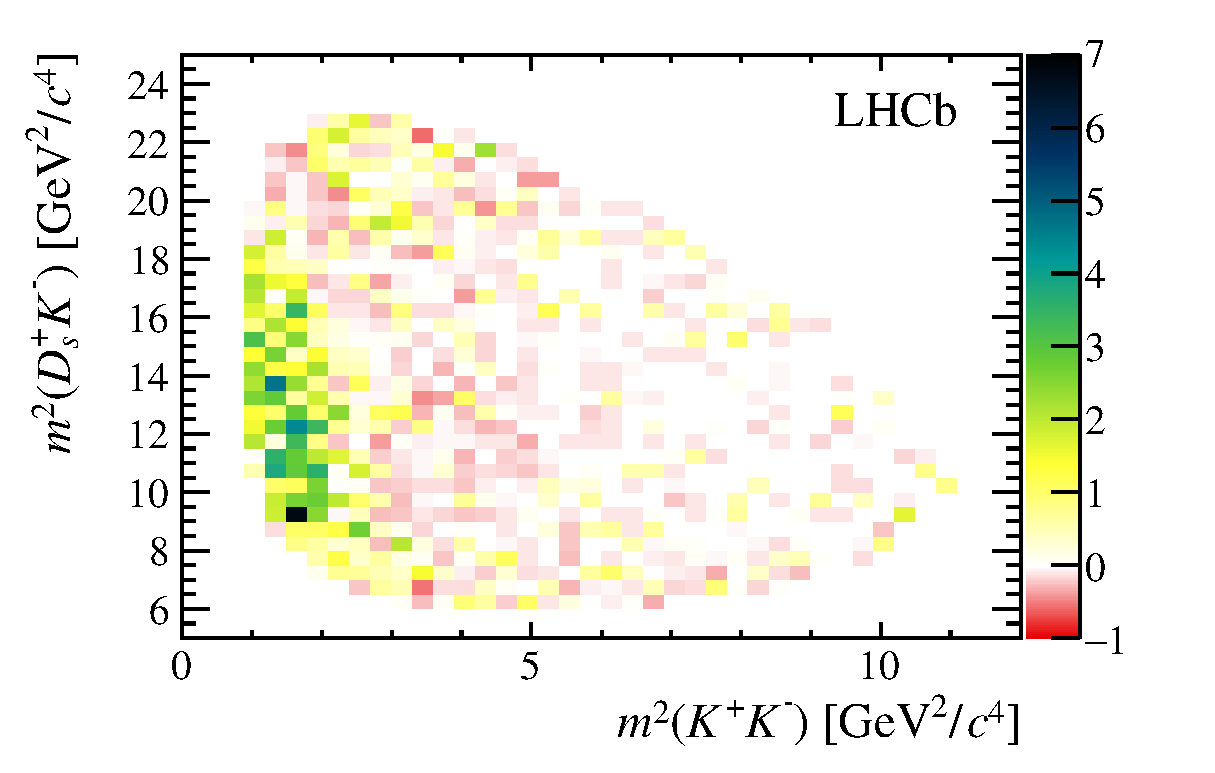
\includegraphics[width=0.8\textwidth]{figs/B2DsKK/Dalitz_plot_sweighted.eps}
    \caption{Dalitz plot}
    \label{fig:_cls}   
\end{figure}
%%%%%%%%%%%%%%%%%%%%%%%%%%%%%%%%%%%%%%%%%%%%%%%%%%%%%%%%%%

%%%%%%%%%%%%%%%%%%%%%%%%%%%%%%%%%%%%%%%%%%%%%%%%%%%%%%%%%%
\begin{figure}[!h]
    \centering
    \begin{subfigure}[t]{0.49\textwidth}
        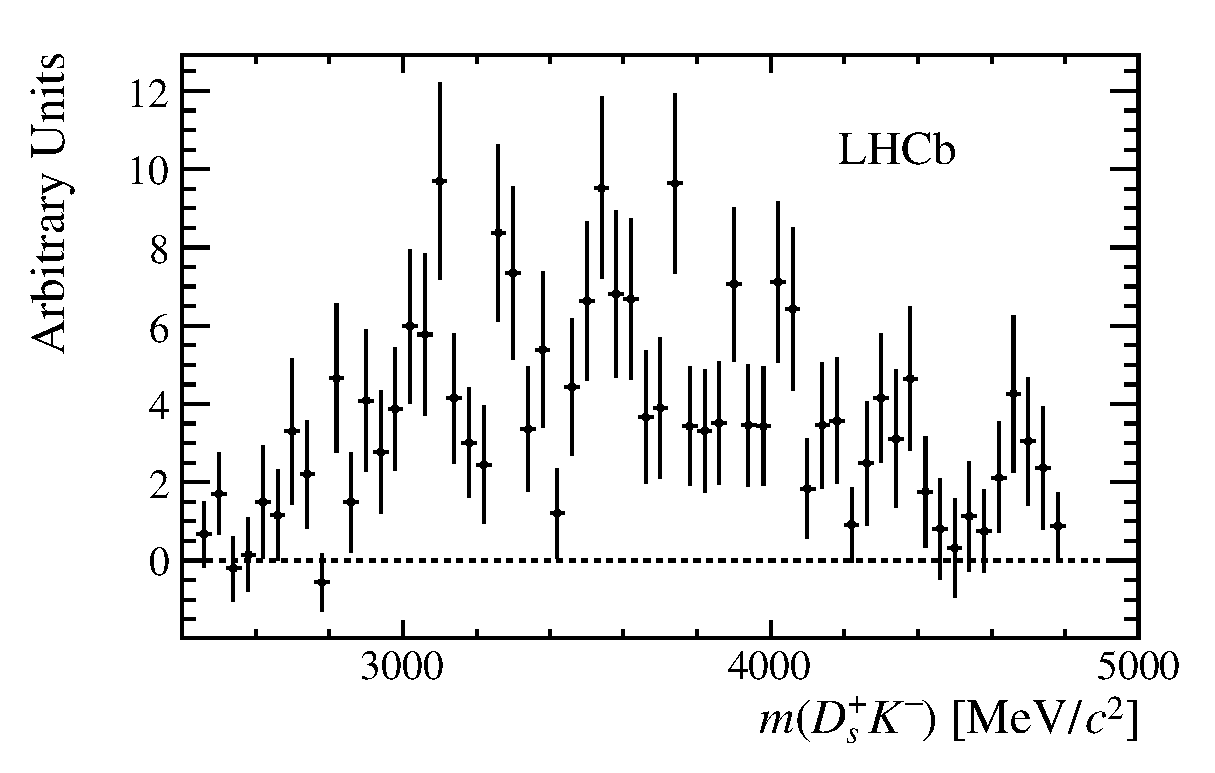
\includegraphics[width=1.0\textwidth]{figs/B2DsKK/DsKm_mass_sweighted.eps}
        %\caption{Normalisation without selection}
    \end{subfigure}
    \begin{subfigure}[t]{0.49\textwidth}
        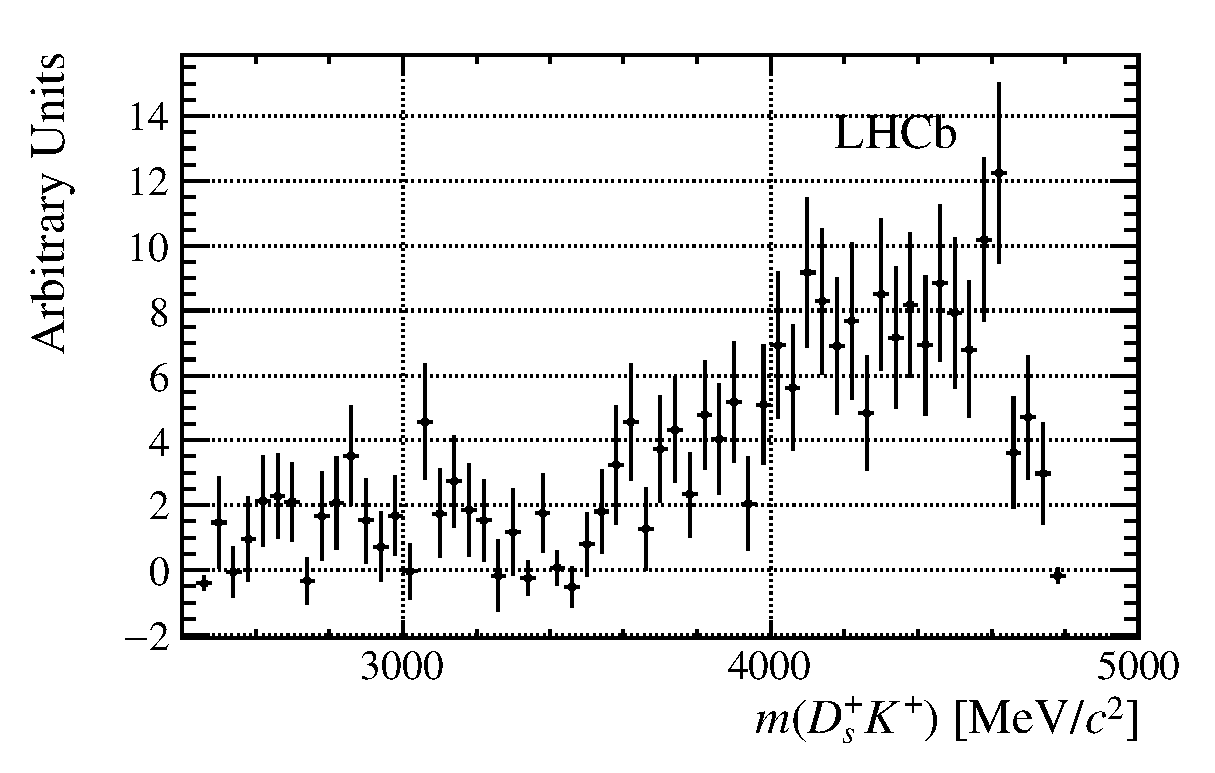
\includegraphics[width=1.0\textwidth]{figs/B2DsKK/DsKp_mass_sweighted.eps}
        %\caption{Normalisation without selection}
    \end{subfigure}
    \begin{subfigure}[t]{0.49\textwidth}
        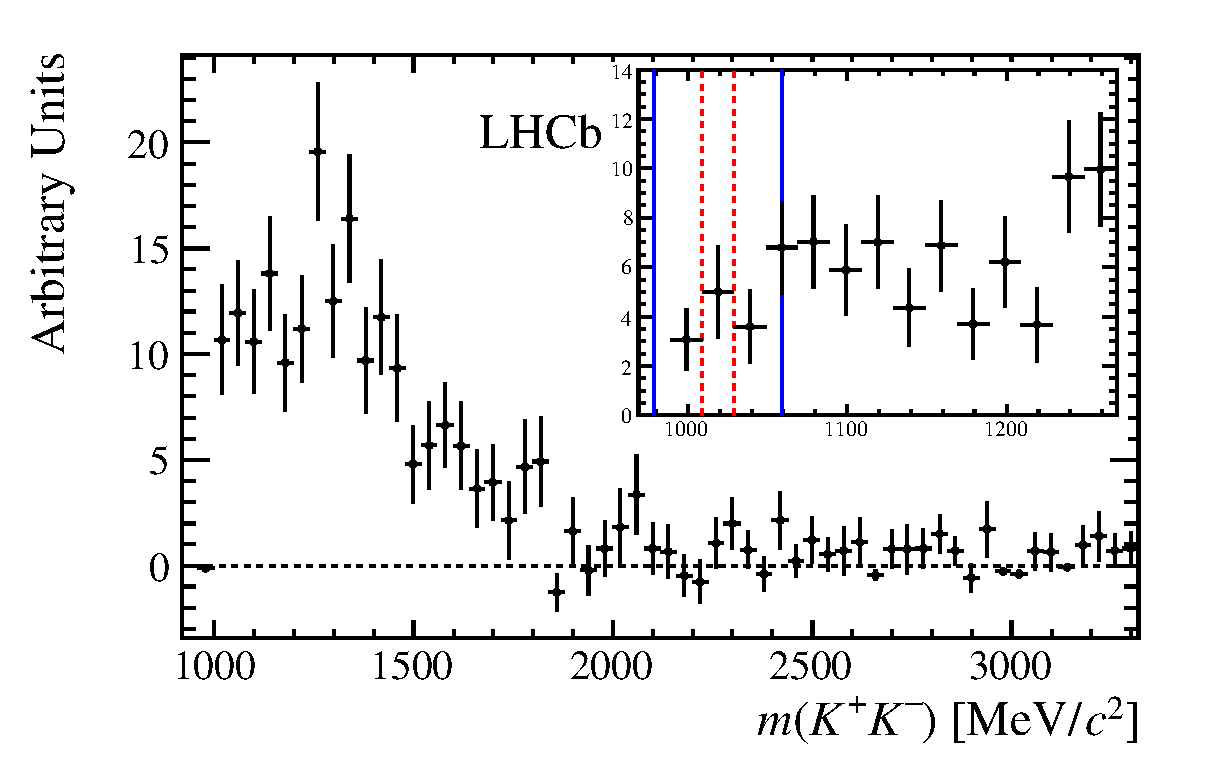
\includegraphics[width=1.0\textwidth]{figs/B2DsKK/phi_mass_sweighted.eps}
        %\caption{Normalisation without selection}
    \end{subfigure}
    \caption{Two-body mass projections}
\end{figure}
%%%%%%%%%%%%%%%%%%%%%%%%%%%%%%%%%%%%%%%%%%%%%%%%%%%%%%%%%%

